\chapter{Problem Definition and Algorithms} \label{ch:algorithms}
	In this chapter, we introduce a practical procedure to implement the Blockchain methodology in a temporal relational database as well as the principles to verify trustworthiness of the records and Blockchain. Then we talk about creating snapshots of relations using the temporal database. In that section we fomally define the problem of large query workload inefficiency in the context of temporal relational databases and then we propose a solution to lower the cost of such queries. Majority of the definitions, figures, examples and discussions used for the topic of snapshot materialization of this chapter were borrowed from our paper in \cite{beirami2018snapshot}.

	\section{Development of Blockchain-based temporal relations} \label{sec:temporal_blockchain}
		In this section we extensively talk about the implementation of Blockchain for the temporal relational database. The first step towards this objective is to augment some attributes to the relations that hold the security information of the records.

		\subsection{Temporal table with security information} \label{sec:temporal_with_security}
		The first step towards building a temporal table with security information is to generate a pair of Cryptographic keys $\langle K_{priv}^u, K_{pub}^u \rangle$ and a unique username for each user of the system. Using the Cryptographic keys, the system is able to create and verify digital signatures of the transactions performed by users. We previousely discussed the generation of digital signatures in \ref{sec:cryptography}. Now we talk about the generation of digital signatures in the context of the proposed temporal database.

			\begin{defn}[digital signature of the transactions] 
				Let $u$ be the user who submitted a set of records $rec_j =\{rec_1,rec_2,...,rec_n\}$ to $r_i^T$. Given the private key of the user denoted as $K_{priv}^u$ the signature of each record could be computed as $$signature(rec_j|K_{priv}^u)= encrypt(hash(rec_j),K_{priv}^u)$$  
			\label{defn:digital_signature}
			\end{defn}

		By storing the digital signature of the records, we provide trustworthy verification for the records. This attempt makes it difficult for the adversaries to forge the records of the database, however the undetectable malicious activities are still possible. In order to add to the difficulty of forgeries on the temporal relation, we tend to create a chain of records using the digital signatures.

			\begin{defn}[Temporal table with Blockchain]
				The temporal relational table with chained security information denoted as $r_i^{T*}$ is a table with the attributes $$attr(r_i^{T*}) = attr(r_i^T) \cup \{username,currentSignature, previousSignature)\}$$ where $username$ is the unique identity of the user who submitted the transaction, currentSignature is the digital signature of the submitted transaction and previousSignature is the signature of the previous record stored in $r_i^T$. 
			\label{defn:temporal_blockchain}
			\end{defn}

			\begin{example} 
				The Table \ref{temporal_blockchain_table} is an example of a temporal relational table with chained security information. With assumption that each record is a block, this table also could be depicted as Figure \ref{fig:blockchain_representation} which is the blockchian representation of Table \ref{temporal_blockchain_table}.
			\label{example:blockchain}
			\end{example}

			\begin{center}
			\begin{table}
				\centering
				\footnotesize
				\caption{Temporal Table $r_1^T$ with chained security information}
				\label{temporal_blockchain_table}
				\begin{tabular}{p{0.5cm}p{0.5cm}p{1cm}p{0.5cm}p{1.7cm}p{1.7cm}p{1.5cm}p{1.5cm}p{1.5cm}}
					\hline
					r\_id & id & item      & value  & timestamp  & deleted & username & curSgn & prevSgn \\ \hline
					151& 21 & Ruler    & 3.25  & 2018-02-10  &  False & Bob &r3T49TR & 0\\  
					152& 21 & Ruler    & 3.25  & 2018-02-20  & True  & Alice & yu0PmER & r3T49TR\\
					153& 22 & Pencil    & 8.0  & 2018-03-21  &  False & Alice & gI90vjN & yu0PmER\\
					154& 23 & Pen    & 12.0  & 2018-03-30  &  False & Bob & 89Ec578 & gI90vjN\\
					155& 22 & Pencil & 7.50  & 2018-04-01 & False & Eve & Ipu32h6 & 89Ec578\\ \hline
				\end{tabular}
			\end{table} 
			\end{center}

			\begin{figure}
				\centering
				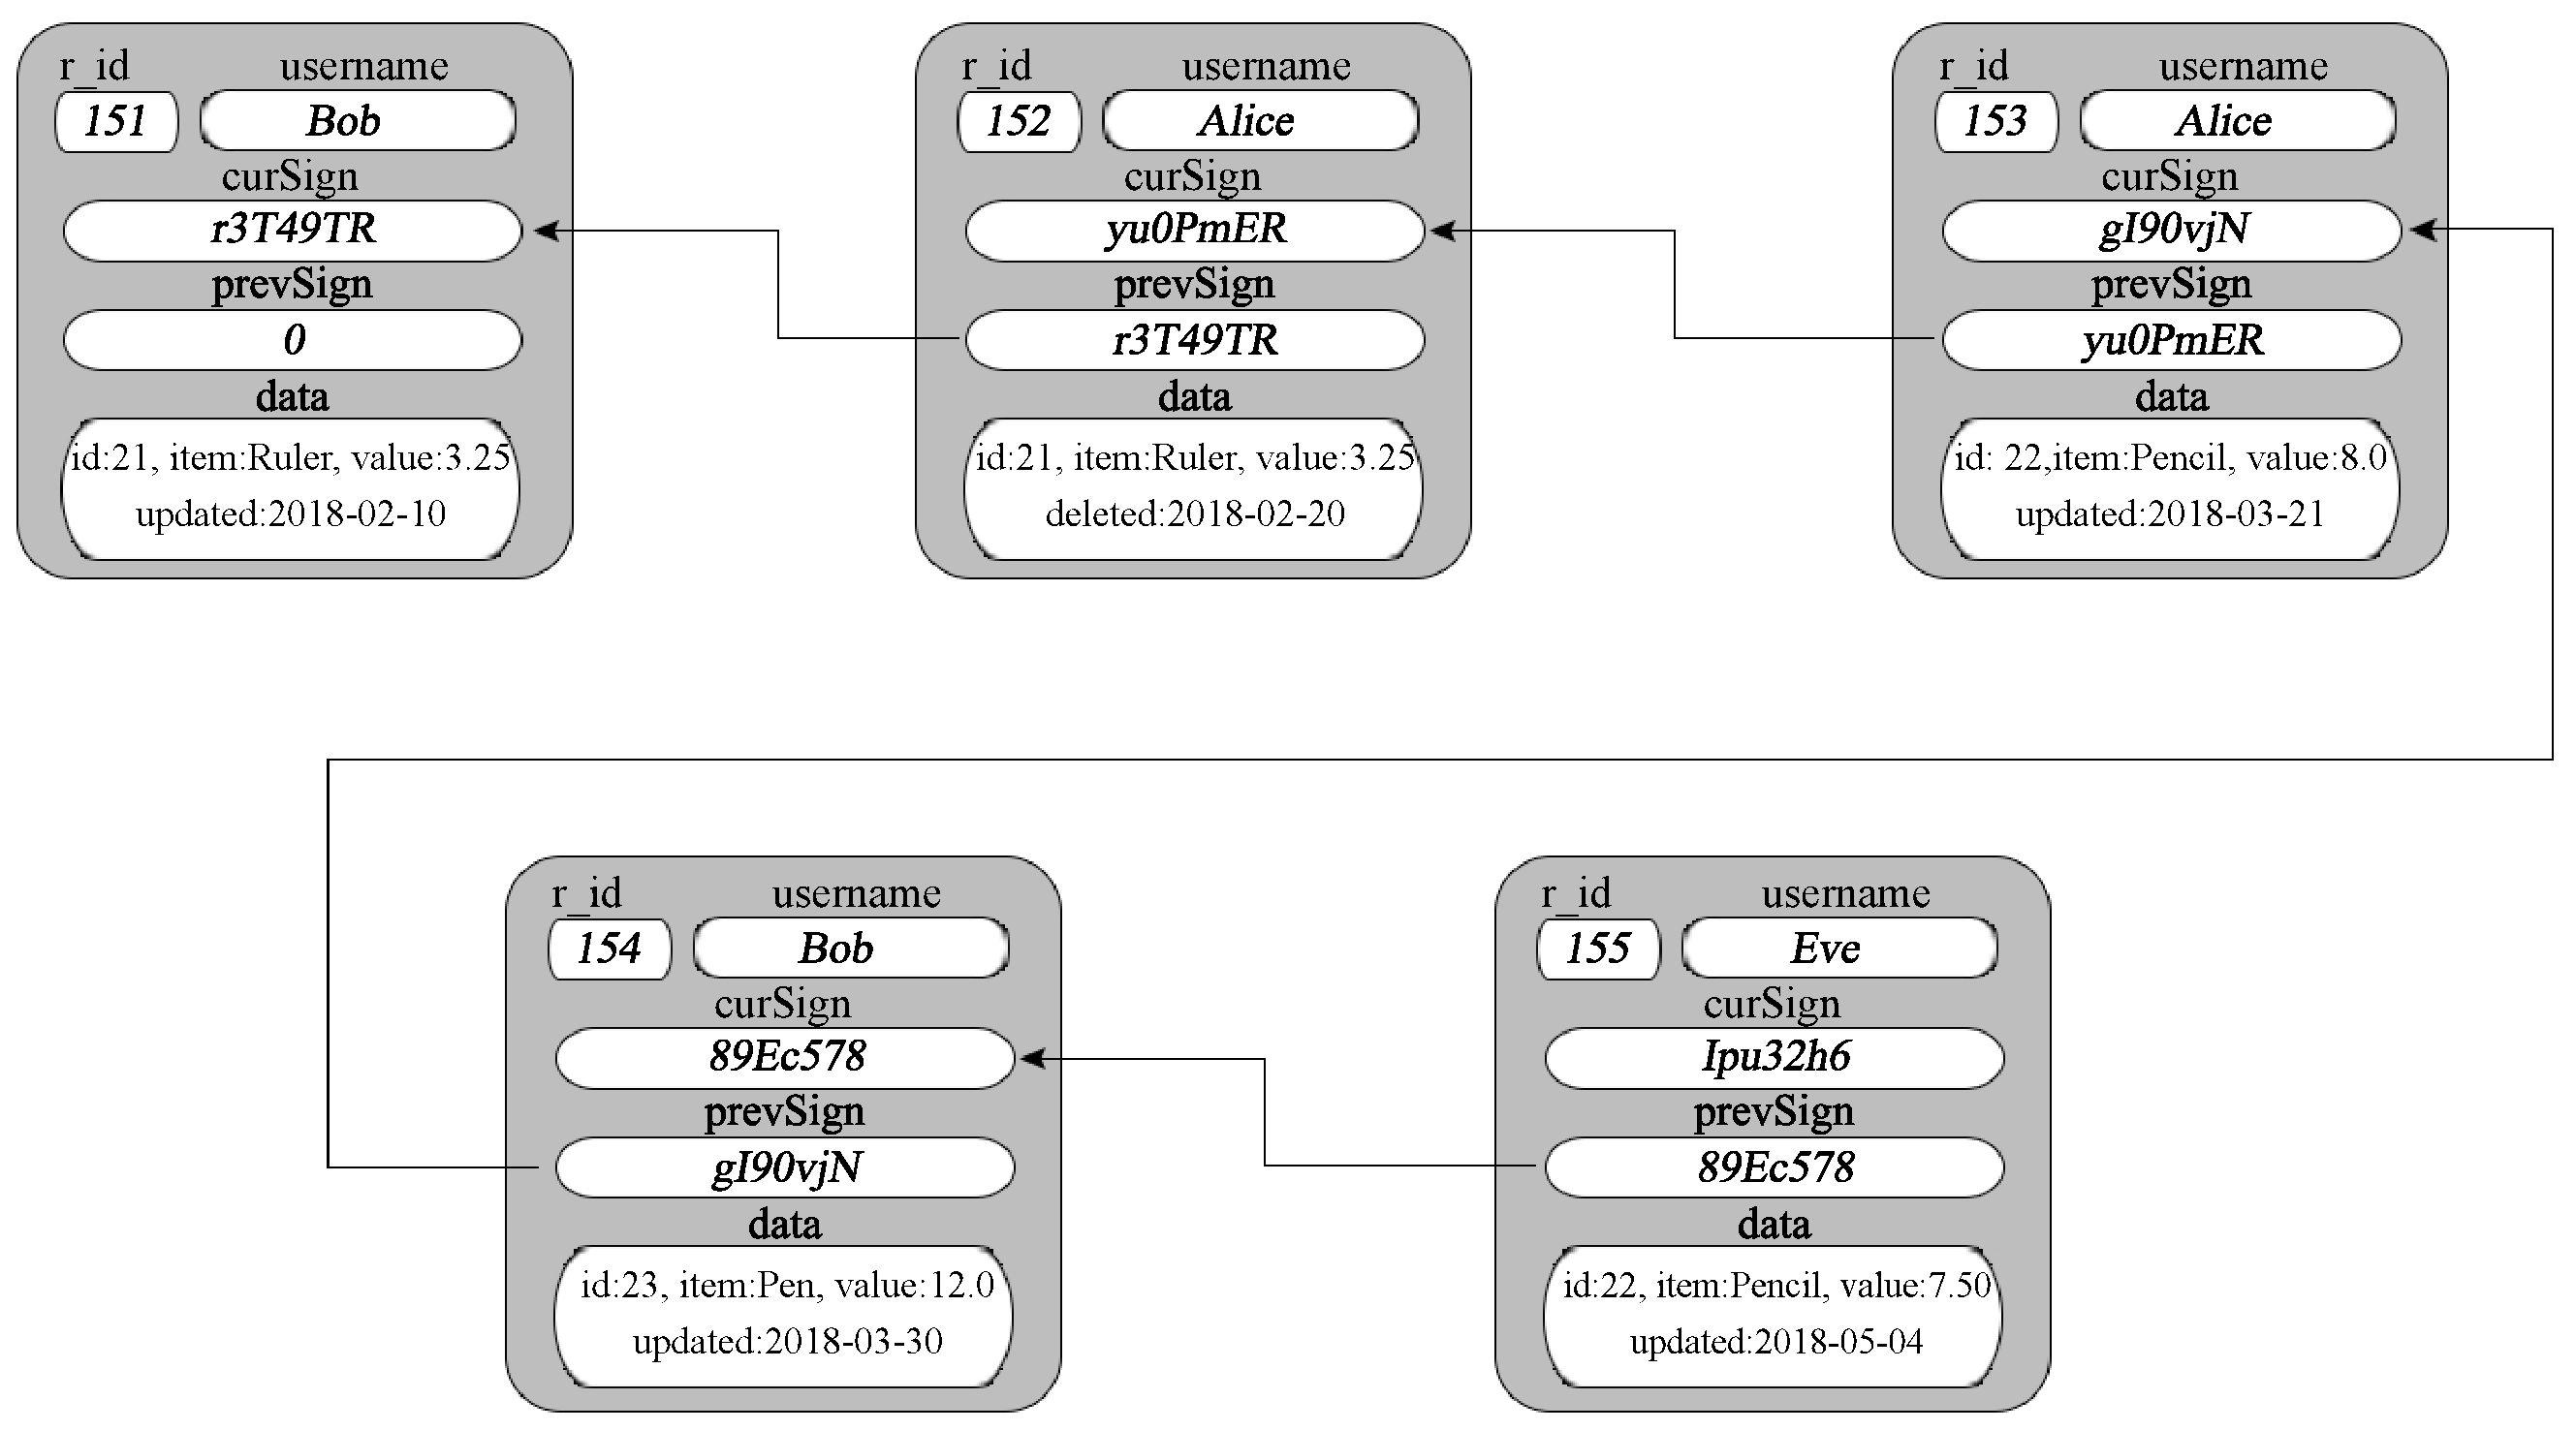
\includegraphics[width=\textwidth]{figs/temporal_blockchain.pdf}
				\caption{Blockchain representation of the table $r_1^T$.}
				\label{fig:blockchain_representation}
			\end{figure}


			\begin{defn}[Chain verification]
				To verify if a chain of the records are valid, the following steps are proposed:
				\begin{itemize}
					\item \textbf{step 1.} verify the $currentSignature$ of individual records.
					\item \textbf{step 2.} check if $rec_j[previousSignature] == rec_{j-1}[currentSignature]$ except for $rec_0$
				\end{itemize}
			\label{chain_verification}
			\end{defn}

			A chain is said to be broken if inconsistent information being gained in any of the above steps. The process of chain verification could also be rewrittem as Algorithm \ref{alg:blockchain_verification}.

			\begin{figure}[h]
				\begin{algorithm}[H]
					\SetAlgoLined
					\caption{Blockchain verification}
					\SetAlCapNameFnt{\tiny}
					\label{alg:blockchain_verification}
					\DontPrintSemicolon
					 \SetKwFunction{FMain}{blockchainVerification}
					 \SetKwProg{Fn}{Function}{:}{}
					 \Fn{\FMain{$last\_id$}}{
					    \For{$i \gets 1$ \KwTo $last\_id$}{
		    				publicKey $\gets$ SELECT publicKey FROM USERS WHERE user = username;\;
					    	$validity$ = verifySign($rec_i$,signature,publicKey)\;
							\uIf{validity != $valid$}{
								\Return Broken chain \;
								\textbf{Break}\;
							}
							\uIf{$rec_i$[$prev\_sgn$] != $rec_{i-1}$[$signature$]}{
								\Return Broken chain \;
								\textbf{Break}\;
							}

					    }
					    \Return Valid Chain
					}
				\end{algorithm} 
			\end{figure}

		\subsection{Appending transactions} \label{ch:append_of_transactions}
		We previousely talked about how to provide security information for the records of the temporal relations. In order to append a transaction along with its security information to these temporal relations, the following steps should be taken:
		\begin {itemize}
			\item First the triggers of the database detect transactions on the records of the database.
			\item The transaction submitter's information is retrived from the users table.
			\item The position of the updated record on the temporal table is determined and the digital signature of its previous record is retrieved.
			\item A digital signature of the updated record concatinated with its previous record's digital signature is computed by utilizing the transaction submitter's cryptographic keys.
			\item The updated record is appended at the end of the table and chained to the end of blockchain by pointing to its previous record's digital signature.
		\end{itemize}
		
		\begin{prop}[incremental manitenance of blockchain cost] 
			By assuming that the updates $\delta D$ on the temporal database occur in constant time, appending these updates to the end of blockchain is done in a constant time $\mathcal{O}(\delta D)$.
		\end{prop}

		It is not realistic to assume that all the transactions in a database system occur in separate timestamps. In fact when concurrent transactions are performed, a database system without concurrency control, has no preference to decide which transaction to be submitted first, therefore it may result in an inconsistent database and consequently an inconsistent blockchain. 

		To solve the issue of concurrent transactions on the database, the transactions on the database need to be {\it serializable}. Serializability grants some order to the execution of concurrent transactions on the database system. This could be achieved by utilizing either the inherent to relational database engine concurrency control tools or software-based alternatives such as software transactional memory. In this project we utilized {\it serializable} isolation level that is defined by SQL standards and supported by Postgresql database to provide serializability for the concurrent transactions on the database system.



	\section{Snapshot creation} \label{sec:problem_def}

		Our proposed trusted temporal database provides data provenance for the records that are stored in a relational database. Given a temporal relation, for the sake of decision making and data analytics, it is common to query for the version of a relation in an specific timestamp. These queries could be answered by creating snapshot of the relation using temporal database.


		\begin{prop}[Linear time in creating snapshots]
			Given a relation $r$, we are interested to create a snapshot of this relation at time $t$, using the temporal relation $r^T$. Assume that the table was updated at a constant rate over time, then the complexity of $\mathrm{snapshot}(r, t)$ is $$\mathcal{O}(|\{x: x\in r^T\mathrm{\ and\ } x.\mathrm{updates} \leq t\}|)\simeq \mathcal{O}(t)$$ 
		\label{prop:linear_time}
		\end{prop}
			Creating snapshots from timeline perspective could be depicted in Figure \ref{fig:snapshot_notion}.
			Also the records that need to evaluated to create a snapshot can be shown in Figure \ref{fig:checked_records}. This clearly shows that computing a snapshot requires visiting each record that has been submitted before $t$ once, and apply the updates. The problem is that, as the number of records to be evaluated grow, creating snapshot become computationally more expensive.

		\begin{figure}
			\centering
			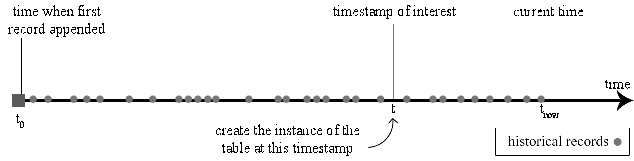
\includegraphics[width=\textwidth]{figs/snapshot_notion.pdf}
			\caption{The notion of creating snapshot on the timeline.}
			\label{fig:snapshot_notion}
		\end{figure}

		\begin{figure}
			\centering
			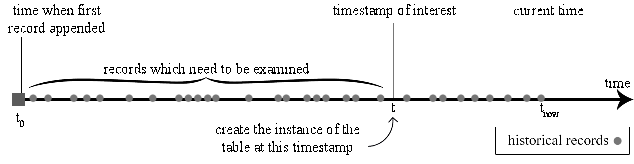
\includegraphics[width=\textwidth]{figs/tobechecked_records.pdf}
			\caption{The records which needs to be checked when creating a snapshot.}
			\label{fig:checked_records}
		\end{figure}

		

		\subsection{Query answering using materialized snapshots} \label{sec:query_using_snapshots}
			Using pre-computed materialized view has been proven to be effective in reducing the computational time of query answering \cite{sohrabi2016materialized} \cite{du2017deepsea}.  As discussed earlier, running queries $Q(t)$ on temporal table $r^T$ to build snapshots and verifying its Blockchain requires linear time with time complexity of approximately $\mathcal{O}(t)$. Consequently in the presence of multiple and concurrent queries, such transactions are computationally expensive and inefficient. We argue that, if a snapshot is computed at an specific timestamp $t$ and placed on the timeline for materialization, the computational time of answering to the subsequent queries on $r^T$ is reduced. The notion of having precomputed snapshots for materialization can be depicted as Figure \ref{fig:snapshot_materialization}. Note that the snapshot could exist before or after a query and in both cases, the query can use the snapshot for materialization.

			\begin{figure}
				\centering
				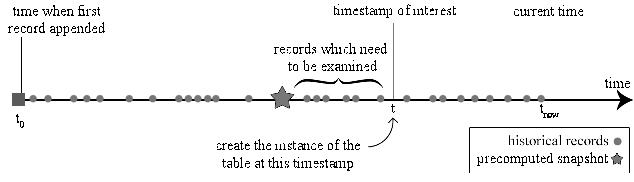
\includegraphics[width=\textwidth]{figs/snapshot_materialization.pdf}
				\caption{The records which needs to be checked when creating a snapshot with having a precomputed snapshot for materialization.}
				\label{fig:snapshot_materialization}
			\end{figure}

			\begin{prop}
				suppose we have a precomputed snapshot $s$ that is placed on the timeline for materialization. Then creating $snapshot(r,t)$ can be computed with complexity:
				$$\mathcal{O}(|\{x: x\in r^T\mathrm{\ and\ } x.\mathrm{updates} \in [s,t]\}|) \simeq \mathcal{O}(|s-t|)$$
				where $t$ is the timestamp of interest.
			\label{prop:materialized_snapshot_complexity}
			\end{prop}

			\begin{example}
				Given a temporal relational table $r_1^T$ (Table \ref{table:temporal_table_3}) and a precomputed snapshot table $s_1$ at timestamp $t = 2018-03-11$(Table \ref{table:snapshot_s1}), we are interested to create a snapshot $s_2$ which is the instance of table $r_1$ at the timestamp of $t = 2018-03-15$. In order to compute snapshot $s_2$, Table \ref{table:transactions_nonmaterialized} shows the transactions which needs to be evaluated without using snapshot $s_1$ and Table \ref{table:transactions_nonmaterialized} is when $s_1$ is used for materialization. This example clearly shows that when creating snapshot $s_2$ (Table \ref{table:snapshot_s2}), less transactions need to be evaluated when $s_1$ is used for materialization.
			\label{example:materialized_snapshot_complexity}
			\end{example}

			\begin{center}
			\begin{table}
				\centering
				\caption{Temporal Table $r_1^T$}
				\label {table:temporal_table_3}
				\begin{tabular}{p{1cm}p{2cm}p{3cm}p{3cm}p{2cm}}
					\hline
					id & item & value  & timestamp  & deleted\\ \hline
					1 & Paper & 0.25  & 2018-02-10  &  False \\  
					2 & Scissors & 8.0  & 2018-02-12  &  False \\
					3 & Folder & 1.50  & 2018-02-12  &  False \\
					1 & Paper & 0.30  & 2018-02-13  &  False \\
					4 & Pencil & 3.0  & 2018-02-16  &  False \\
					3 & Folder & 1.75  & 2018-02-21  &  False \\
					5 & Batteries & 8.0  & 2018-02-23  &  False \\
					1 & Paper & 0.35  & 2018-02-25  &  False \\
					6 & Notebook & 7.0  & 2018-03-01  &  False \\
					5 & Batteries & 9.0  & 2018-03-01  &  False \\
					4 & Pencil & 3.25  & 2018-03-04  &  False \\
					1 & Paper & 0.35  &  2018-03-04 & True \\
					7 & Ruler & 4.0  & 2018-03-06  &  False \\
					2 & Scissors & 8.50  & 2018-03-07  &  False \\
					7 & Ruler & 4.50  & 2018-03-08  &  False\\
					5 & Batteries & 11.0  & 2018-03-10 & False \\
					3 & Folder & 1.75  & 2018-03-11 & True \\
					7 & Ruler & 4.50  & 2018-03-12  & True  \\
					6 & Notebook & 7.50  & 2018-03-15 & False \\ 
					2 & Scissors & 7.50  & 2018-03-17 & False \\ \hline
				\end{tabular}
			\end{table}
			\begin{table}
				\centering
				\caption{Snapshot $s_1$ at $t = 2018-03-11$}
				\label{table:snapshot_s1}
				\begin{tabular}{p{4cm}p{4cm}p{4cm}}
					\hline
					id & item  & value  \\ \hline
					2 & Scissors & 8.5   \\ 
					4 & Pencil & 3.25   \\ 
					5 & Batteries & 11.0   \\ 
					6 & Notebook & 7.0 \\ 
					7 & Ruler & 4.50   \\ \hline
				\end{tabular}
			\end{table}
			\end{center}

			\begin{center}
			\begin{table}
				\centering
				\caption{the transactions to compute snapshot $s_2$ at $t = 2018-03-15$ without using snapshot $s_1$ for materialization}
				\label{table:transactions_nonmaterialized}
				\begin{tabular}{p{1cm}p{2cm}p{2cm}p{3cm}p{2cm}p{2cm}}
					\hline
					id & item & Transaction  &timestamp & value  &query on\\ \hline
					1 & Paper & cretaed & 2018-02-10 & 0.25 & $r_1^T$ \\
					  & Paper & updated & 2018-02-13 & 0.30 & $r_1^T$ \\
					  & Paper & updated & 2018-02-25 & 0.35 & $r_1^T$ \\
					  & Paper & deleted & 2018-03-04 & - & $r_1^T$ \\ \hline
					2 & Scissors & cretaed & 2018-02-12 & 8.0 & $r_1^T$ \\
					  & Scissors & updated & 2018-03-07 & 8.50 & $r_1^T$ \\ \hline
					3 & Folder & cretaed & 2018-02-12 & 1.50 & $r_1^T$ \\
					  & Folder & updated & 2018-02-21 & 1.75 & $r_1^T$ \\
					  & Folder & deleted & 2018-03-11 & - & $r_1^T$ \\ \hline
				  	4 & Pencil & cretaed & 2018-02-16 & 3.0 & $r_1^T$ \\
					  & Pencil & updated & 2018-03-04 & 3.25 & $r_1^T$ \\ \hline
			  	  	5 & Batteries & cretaed & 2018-02-23 & 8.0 & $r_1^T$ \\
					  & Batteries & updated & 2018-03-01 & 9.0 & $r_1^T$ \\
					  & Batteries & updated & 2018-03-10 & 11.0 & $r_1^T$ \\ \hline
					6 & Notebook & cretaed & 2018-03-01 & 7.0 & $r_1^T$ \\ 
					  & Notebook & updated & 2018-03-15 & 7.50 & $r_1^T$ \\ \hline
					7 & Ruler & cretaed & 2018-03-06 & 4.0 & $r_1^T$ \\
					  & Ruler & updated & 2018-03-08 & 4.50 & $r_1^T$ \\
					  & Ruler & deleted & 2018-03-12 & - & $r_1^T$ \\ \hline

				\end{tabular}
			\end{table}
			\end{center}

			\begin{center}
			\begin{table}
				\centering
				\caption{the transactions to compute snapshot $s_2$ at $t = 2018-03-15$ using snapshot $s_1$ for materialization}
				\label{table:transactions_materialized}
				\begin{tabular}{p{1cm}p{2cm}p{2cm}p{3cm}p{2cm}p{2cm}}
					\hline
					id & item & Transaction  &timestamp & value  &query on\\ \hline
					2 & Scissors & - & - & 8.50 & $s_1$ \\ \hline
				  	4 & Pencil & - & - & 3.25 & $s_1$ \\ \hline
			  	  	5 & Batteries & - & - & 11.0 & $s_1$ \\ \hline
					6 & Notebook & - & - & 7.0 & $s_1$ \\ 
					  & Notebook & updated & 2018-03-15 & 7.50 & $r_1^T$ \\ \hline
					7 & Ruler & - & - & 4.50 & $s_1$ \\
					  & Ruler & deleted & 2018-03-12 & - & $r_1^T$ \\ \hline
				\end{tabular}
			\end{table}
			\end{center}

			\begin{center}
			\begin{table}
				\centering
				\caption{Snapshot $s_2$ at $t = 2018-03-15$}
				\label{table:snapshot_s2}
				\begin{tabular}{p{4cm}p{4cm}p{4cm}}
					\hline
					id & item  & value  \\ \hline
					2 & Scissors & 8.50   \\ 
					4 & Pencil & 3.25   \\ 
					5 & Batteries & 11.0   \\ 
					6 & Notebook & 7.50 \\ \hline
				\end{tabular}
			\end{table}
			\end{center}

	\section{Single snapshot for materialization} \label{sec:optimal_materialization}
		Let $T_q = \{q_1, q_2, \dots, q_n\}$ be the timestamps of $n$ queries, each querying the database at $D^T(q_i)$. To save on computational cost in answering the queries on temporal database $D^T$, we propose to compute snapshot $s$ in optimal timestamp on the timeline to answer to $T_q$ at lower cost. 

		\begin{defn}[Cost of Query Answering with single materialized snapshot] 
			In the presence of a single materialized precomputed snapshot $s$ , the cost of answering the query $T_q$ is calculated as:
			$$\mathrm{cost}(T_q | s) = \sum_{q\in T_q} |q - s|$$
		\label{defn:cost_of_query_answering}
		\end{defn}

		\begin{defn}[Optimal Snapshot placement]: 
		    For the \emph{single snapshot placement} problem, the goal is to find the timestamp $s^*$ such that 
			$$cost(T_q|s)= Arg min(\sum_{q\in T_q}|q - s|)$$
		\label{defn:optimal_snapshot_placement}
		\end{defn}

	\subsection{Optimal single snapshot placement} \label{sec:optimal_single_snapshot}
		 Let $T_q^* = \{q_1,q_2, \dots , q_n\}$ be $n$ number of queries performed on the temporal database. $T_q^*$ gives us a valuable insight into the query patterns on the temporal database, that could be used to find optimal position of snapshots.

		\begin{prop}
			Given the performed queries $T_q^*$, the optimal position for a single snapshot on the timeline for materialization is $s^*(T_q^*)=median(T_q^*)$ that can be computed in $\mathcal{O}(|T_q^*|)$. 
		\label{prop:compute-median}
		\end{prop}
		    
		Figure \ref{fig:optimal_materialization} shows the notion of placing snapshot in the median of queries for materialization.

		\begin{figure}
			\centering
			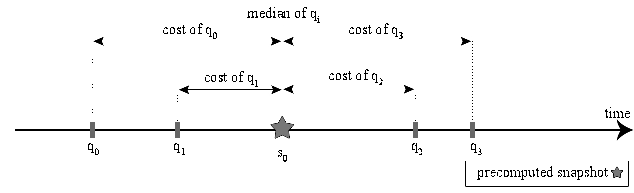
\includegraphics[width=\textwidth]{figs/optimal_materialization.pdf}
			\caption{Placing a single snapshot in the median of queries guarantees the optimal cost of query answering.}
			\label{fig:optimal_materialization}
		\end{figure}

		\textbf{\emph{Proof of the Proposition~\ref{prop:compute-median}}}:
			At first, we solve the problem of a single snapshot placement for two queries, and then we generalize the conclusion for multiple queries:

			Assume that there are two queries $T_q=\{q_1,q_2 \}$ on the timeline, such that, $q_1<q_2$. for the placement of a single snapshot $s^*$ on the timeline, there are several cases which needs to be considered:

			\emph{Case 1}:
			$s^* \in [q_1,q_2]$, hence $q_1\leq s^*\leq q_2$.
			in this case, the cost is:

			$$cost(T_q|s^*)=\sum_{i=1}^2|q_i-s^*| = (s^*-q_1+q_2-s^*)=(q_2-q_1)$$

			from case 1, we can infer that the cost of running two queries $q_1$ and $q_2$ when the snapshot is placed between them, is equal to the deviation between the two queries.

			\emph{Case 2}:
			$s^* \notin [q_1,q_2]$ and $s^* < q_1 < q_2$. for this case the cost could be calculated as follows:
			$$cost_T(T_q|s^*)=\sum_{i=1}^2|q_i-s^*| = (q_1-s^*+q_2-s^*)=(q_1+q_2-2s^*) $$$$>(q_1+q_2-2q_1)=(q_2-q_1)$$

			Therefore we conclude that if the snapshot $s^*$ is placed before queries $T_q$, the cost to perform both queries is greater than when the snapshot is placed between the two queries.

			\emph{Case 3}:
			$s^* \notin [q_1,q_2]$ and $q_1 < q_2 < s^*$.
			$$cost(T_q|s^*)=\sum_{i=1}^2|q_i-s^*| = (s^*-q_1+s^*-q_2)=(2s^*-q_1-q_2) $$$$>(2q_2-q_1-q_2)=(q_2-q_1)$$

			hence, if the snapshot $s^*$ is placed after the queries $T_q$, then the cost of performing those queries are greater than when the snapshot is placed between them.

			From case1, case2 and case3, we can conclude that the optimal timestamp on the timeline that we can place the single snapshot $s^*$ to perform two queries $T_q = \{q_1,q_2\}$, where $q_1<q_2$ is when $s^* \in [q_1,q_2]$.

			Now, we generalize our conclusion from the cases that we evaluated, for the placement of a single snapshot in the presence of $n$ number of queries on the timeline: 

			Suppose that there is a set of queries $T_q=\{q_1,q_2,...,q_n\}$ performed on the timeline. To evaluate the most optimal position to place the single snapshot $s^*$ for materialization, we breakdown the set of queries into the set of nested intervals $[q_1,q_n],[q_2,q_{n-1}],...,[q_i,q_{n+1-i}]$ where $n$ is the number of queries on timeline and $i=0,1,2,...,c$ where $c=\frac{n+1}{2}$ for odd number of queries and $c=\frac{n}{2}$ for even number of queries.

			Based on the conclusion that we obtained from examining case 1, case 2 and case 3 earlier, for each nested interval, the cost of queries inside them is minimized if snapshot $s^*$ is placed in a middle of the interval. Therefore if the snapshot is placed in a position which $s^*\in \{ [q_1,q_n] \wedge [q_2,q_{n-1}] \wedge ... \wedge [q_i,q_{n+1-i}] \}$ the overall cost for all queries is minimized. In other words, if the snapshot is placed in a position that is in the middle of all nested intervals, then the total sum of absolute deviation of the snapshot from all queries is minimized. The placement of snapshot $s^*$ in the median position of $T_q$ guarantees that the snapshot is placed in the middle of all nested query intervals, where the cost of queries is calculated as follows:
			$$cost(T_q|s^*)=\sum_{i=1}^n |q_i-s^*| = $$
			$$[(|q_1-s^*|+|q_n-s^*|)+(|q_2-s^*|+|q_{n-1}-s^*|)+...+|q_c-s^*|+|q_{n+1-c}-s^*|)]=$$
			$$[(s^*-q_1+q_n-s^*)+(s^*-q_2+q_{n-1}-s^*)+...+(s^*-q_c+q_{n+1-c}-s^*)]=$$
			$$[(q_n-q_1)+(q_{n-1}-q_2)+...+(q_{n+1-c}-q_c)]$$\\
			where parenthesis indicate the deviation from endpoints for one of nested intervals. In the case when there are odd number of queries performed on the timeline, the innermost interval is $[q_{\frac{n+1}{2}},q_{\frac{n+1}{2}}]$ and the position of $q_{\frac{n+1}{2}}$ is the optimal position to place snapshot $s^*$. Also when there are even number of queries the innermost interval is $[q_{\frac{n}{2}},q_{\frac{n}{2}+1}]$, therefore if we choose snapshot $s^*$'s position to be at $q_{\frac{n}{2}}\leq s^*\leq q_{\frac{n}{2}+1}$,it guarantees that the snapshot exists inside each of nested intervals, and hence the sum of absolute deviation is minimized. 


	\section{Multiple snapshot placement} \label{sec:optimal_multiple_snapshot} \label{sec:optimal_multiple_snapshot}
		In the presence of thousands of queries on a temporal database with millions of records, having a single snapshot reduces the cost of query answering but it is still insufficient. Therefore, to reduce the overall cost of query answring, optimal timestamps should be computed on the timeline of the temporal database to place snapshots for materialization. In the following section, different approaches to compute the optimal positions on the timeline are discussed.

		\begin{prop}[Cost of query answering with multiple materialized snapshots]
			If multiple snapshots $S=\{s_1, s_2, \dots, s_m \}$ were precomputed and materialized, then 
			$$\mathrm{cost}(T_q|S) = \sum_{q\in T_q} \min\{|q-s| : s\in S\}$$
		\label{prop:cost_of_multiple_snapshots}
		\end{prop}


		\begin{prop}[optimal multiple snapshots for materialization]
			The \emph{$m$-snapshot placement} problem is to compute $m$ number of timestamps $S^*=\{s_1, s_2, \dots, s_m\}$ to place $m$ number of snapshots for materialization, such that 
			$$cost(T_q|S)= Arg min(\sum_{q\in T_q}\{|q - s|:s \in S\})$$
		\label{prop:optimal_multiple_snapshot}
		\end{prop}

		\begin{prop}[Optimal number of snapshots] 
			Let $R$ be the total resources available on the system specified by the system designer to handle the given workload, and $\mathcal{L}$ to be the average snapshot size. the maximum number of snapshots $N$ could be determined by: $$N=R/\mathcal{L}$$
		\label{prop:optimal_number_segmentations}
		\end{prop}

		Now, we examine different approaches to find the optimal timestamps to place snapshots. Let $\mathrm{opt}(Q, m)$ be the optimal $m$-snapshot placements for the query workload $Q$. Denote $Q[i,j] = \{q_i,q_{i+1},...,q_{j-1},q_j\}$.

		\begin{prop}[Segmentation of queries] 
			Given an ordered set of snapshot timestamps $S=\{s_1,s_2,...,s_m\}$, such that $s_i \leq s_{i+1}$, and $n$ number of queries $Q = \{q_1,q_2,...,q_n\}$, snapshots create $m$ number of non-overlapping segments on the queries $Q[1,i_1],Q[i_1+1,i_2],...,Q[i_{m-1},i_m]$ such that queries in the segment $Q[i_j,i_{j+1}]$ use $s_j$ to answer the queries in the optimal query answering strategy.
		\label{prop:segmentation_of_queries}
		\end{prop}
		The notion of creating segmentations is depicted in Figure \ref{fig:segmentation}.

		\begin{figure}
			\centering
			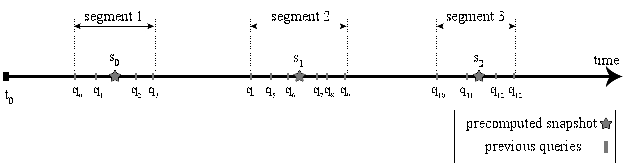
\includegraphics[width=\textwidth]{figs/segmentations.pdf}
			\caption{The notion of creating segmentations on the timeline and placing snapshot for each segmentation.}
			\label{fig:segmentation}
		\end{figure}


		\begin{prop}[Optimality of sub-problems]
			Let $S^* = \mathrm{opt}(Q, m)$.  Let $\mathcal{Q}$ be the partition of segments created by $S^*$.  Then, the prefix of $S^*$ is also an optimal $m-1$ snapshot placement of the prefix of $\mathcal{Q}$. Formally, $$\mathrm{prefix}(S^*) = \mathrm{opt}(\cup\mathrm{prefix}(\mathcal{Q}), m-1)$$
		\label{prop:optimality_of_subproblems}
		\end{prop}

		\subsection{recursive approach to find optimal segmentations of the timeline} \label{sec:optimal_recursive_segmentation}
			We can formulate a recursive definition of $\mathrm{opt}(Q, m)$ using Proposition~\ref{prop:optimality_of_subproblems}. The intuition is that we try out all possible {\em last} segment of $Q$, and pick the one with the lowest cost.

			The recursive definition of $\mathrm{opt}(Q, m)$ is given as:

			\begin{itemize}
				\item Base case $ \mathrm{opt}(Q, 1) = \{\mathrm{median}(Q)\}$.
				\item Induction on $m$:
				$$i^* = \mathrm{argmin}\{\mathrm{cost}(\mathrm{opt}(Q[1,i], m-1)): i\in[1,
				n]\}$$
				$$
				\mathrm{opt}(Q, m) = \mathrm{opt}(Q[1, i^*]) \cup \{\mathrm{median}(Q[i^*+1, n])
				$$
			\end{itemize}
			The recursive formulation of $\mathrm{opt}(Q, m)$ requires $\mathcal{O}(2^{m})$.

			\begin{example}
				Given the queries $Q=\{q_1=2,q_2=4,q_3=9,q_4=11,q_5=17,q_6=20\}$ (Figure \ref{fig:example_recursive_queries}) and maximum number of snapshots $m=3$, the goal is to find the most optimal segmentations using recursive algorithm to place snapshots for materialization. The steps to compute $m$ number of optimal segmentations is shown in Figure \ref{fig:example_recursive_steps}. In this example, the most optimal segmentation possible for 3 snapshots is when $segment_1 = \{q_0,q_1\}$, $segment_2 = \{q_2,q_3\}$, $segment_3= \{q_4,q_5\}$ where the total cost is 7 units. Figure \ref{fig:example_recursive_segmentation}.
			\label{example:recursive_segmantation}
			\end{example}

			\begin{figure}
				\centering
				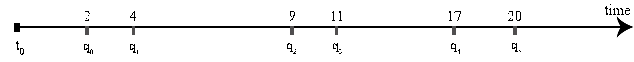
\includegraphics[width=\textwidth]{figs/example_recursive_q.pdf}
				\caption{The quer on the timeline in Example.}
				\label{fig:example_recursive_queries}
			\end{figure}

			\begin{figure}
				\centering
				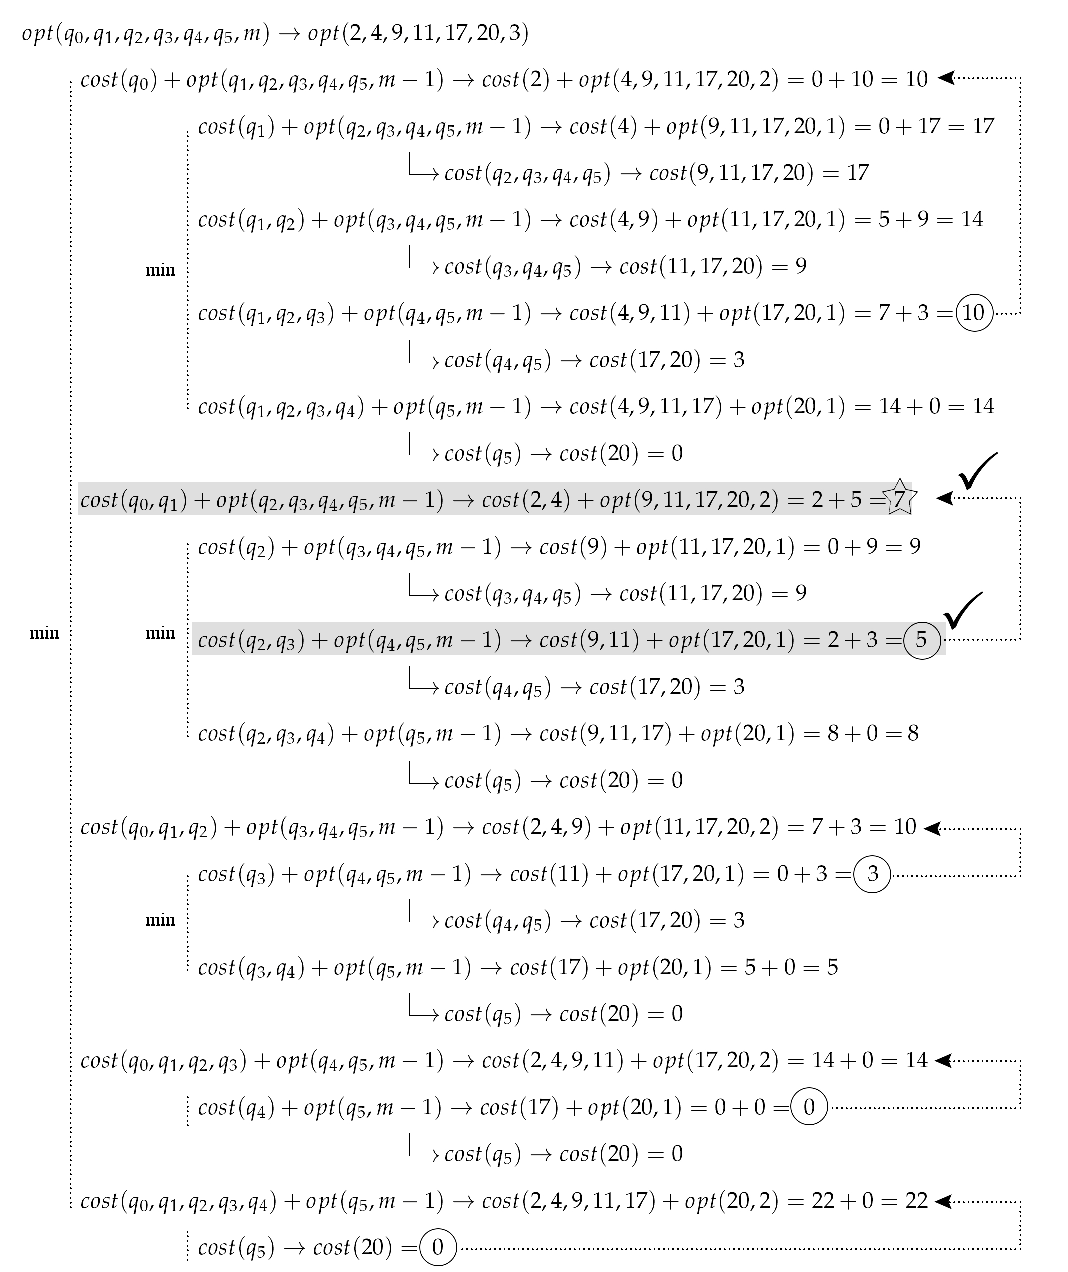
\includegraphics[width=\textwidth]{figs/recursion_example.pdf}
				\caption{Recursive approach to compute optimal segmentations for 3 snapshots.}
				\label{fig:example_recursive_steps}
			\end{figure}


			\begin{figure}
				\centering
				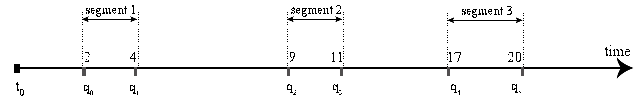
\includegraphics[width=\textwidth]{figs/example_recursive_s.pdf}
				\caption{Segmentation of queries on the timeline for Example \ref{example:recursive_segmantation}}
				\label{fig:example_recursive_segmentation}
			\end{figure}


		\subsection{Dynamic programming approach to find optimal segmentation of the timeline} \label{sec:dynamic_programming_optimal_segment}

			Dynamic programming improves the time complexity of finding optimal segmentations in recursive algorithm by utilizing memoization technique \cite{johnsonbaugh2003algorithms}. In the memoization technique, if the cost of a segmentation is calculated, it is stored in a table where the recursive calls can look up the results in the table instead of recalculating them. We can build a table $\mathbf{OPT}$ as a two dimensional array
			indexed by $(i, k)$ where $i\in [1, n]$ and $k\in [1, m]$.  Each entry
			in the table $\mathbf{OPT}[i,k] = \mathrm{opt}(Q[1,i], k)$.
			We can compute $\mathbf{OPT}[i,k]$ in a bottom up fashion \cite{kossmann2000iterative}.
			The complexity of computing all the entries of $\mathbf{OPT}$ is $\mathcal{O}(mn^2)$.

			\begin{example}
				Given a set of queries $Q={q_0=2,q_1=4,q_2=9,q_3=11}$, we want to compute 3 segmentations from these queries, such that putting a snapshot in each segmentation, make the overall cost of answering to the queries optimal. The process of computing optimal snapshots is  shown in Table \ref{table:dynamic_programming}. This method is more efficient than recursive algorithm as for example in the memoization table T[3][2], the recursive call uses the cost stored in T[2][1], T[2][2] and T[2][3] without the need to recalulate them. In this example, the most optimal overall cost is 2 which is achieved by either $\{segment1 =[q_0,q_1],segment2=[q_2],segment3=[q_3]\}$ or $\{segment1 =[q_0], segment2 = [q_1], segment3 = [q_2, q_3]\}$
			\label{example:dynamic_programming}
			\end{example}

			\begin{table}[]
			\scriptsize
			\renewcommand{\arraystretch}{2}
			\setlength\tabcolsep{1pt}
			\caption{Memoization table T for dynamic programming approach to compute 3 optimal segmentations from 4 queries.}
			\label{table:dynamic_programming}
			\begin{tabular}{|l|l|l|l|l|}
			\hline
			0 & 0 & 0 & 0 & 0 \\ \hline

			0 & $T{[}0{]}{[}0{]}+cost(q_0)$& 
			$T{[}0{]}{[}1{]}+cost(q_0,q_1) $ & 
			$T{[}0{]}{[}2{]}+cost(q_0,q_1,q_2)$&   
			$T{[}0{]}{[}3{]}+cost(q_0,q_1,q_2,q_3) $ \\ 
			 & $0+0 = 0$ & $0+2 = 2$ & $0+7=7$ & $0+14 = 14$ \\ \hline

			0 & 
			$T[1][0]+cost[q_0]$ & 
			$min\left\{\begin{array}{ll}T[1][1]+cost[q_1] \\ T[1][2]+cost[]\end{array}\right.$&
			$min\left\{\begin{array}{lll}T[1][1]+cost[q_1,q_2] \\ T[1][2]+cost[q_2] \\ T[1][3]+cost[] \end{array}\right.$&
			$min\left\{\begin{array}{llll}T[1][1]+cost[q_1,q_2,q_3] \\ T[1][2]+cost[q_2,q_3] \\ T[1][3]+cost[q_3] \\ T[1][4]+cost[] \end{array}\right.$\\ 

			& $0+0 = 0$ & 
			$min\left\{\begin{array}{ll}  0+0 = 0 \\ 0 + 2 = 2 \end{array}\right.$ & 
			$min\left\{\begin{array}{lll}  0+5 = 5 \\ 2 + 0 = 2 \\ 7+0=7  \end{array}\right.$ & 
			$min\left\{\begin{array}{lll}  0+7 = 7 \\ 2 + 2 = 4 \\ 7+0=7 \\ 14+0 = 14 \end{array}\right.$ \\ \hline

			0 & 
			$T[2][0]+cost[q_0]$ & 
			$min\left\{\begin{array}{ll}T[2][1]+cost[q_1] \\ T[2][2]+cost[]\end{array}\right.$&
			$min\left\{\begin{array}{lll}T[2][1]+cost[q_1,q_2] \\ T[2][2]+cost[q_2] \\ T[2][3]+cost[] \end{array}\right.$&
			$min\left\{\begin{array}{llll}T[2][1]+cost[q_1,q_2,q_3] \\ T[2][2]+cost[q_2,q_3] \\ T[2][3]+cost[q_3] \\ T[2][4]+cost[] \end{array}\right.$\\ 

			& $0+0 = 0$ & 
			$min\left\{\begin{array}{ll}  0+0 = 0 \\ 0 + 0 = 0 \end{array}\right.$ & 
			$min\left\{\begin{array}{lll}  0+5 = 5 \\ 0 + 0 = 0 \\ 2+0=2  \end{array}\right.$ & 
			$min\left\{\begin{array}{lll}  0+7 = 7 \\ 0 + 2 = 2 \\ 2+0=2 \\ 4+0 = 4 \end{array}\right.$ \\ \hline

			\end{tabular}
			\end{table}


		\subsection{Heuristic method to find optimal timeline segmentation} \label{sec:heuristic_optimal}
			In the heuristic technique, the optimal solution to a problem is not guaranteed however it could be seen as a suitable alternative solution when runtime has more priority than the accuracy of the solution. For the purpose of finding the optimal segmentation of queries for optimal query answering, we utilized K-means clustering technique. We chose K-means clustering over other clustering methods because each centroids resulted from this technique are in the middle of their cluster, hence they are good candidate to place the snapshots for materialization.

			\begin{prop} 
				Given $T_q^* = \{q_0,q_1,...,q_n\}$ as $n$ number of queries performed on the temporal relation $r^T$, we would like to group the $q_i \in T_q^*$ into $m$ number of \textit{"clusters"}. 
			\label{prop:heuristic_method}
			\end{prop}

			Applying K-means clustering methodology to this problem requires to minimize the objective function defined as:
			$$J = \sum_{j=1}^{m} \sum_{i=1}^{n} ||q_i^{(j)}-\mu_j||^2$$
			where $\mu_j$ is the centroid of $j^{th}$ cluster and $||q_i^{(j)}-\mu_j||^2$ is the squared error function which indicates the distance between each query and their assigned centroids.
			Minimizing objective function is achieved by the relocation of $\mu_j$ until no changes occur in the objective function.



	
		\section{Trusted Snspshots for materialization} \label{sec:trusted_snapshots}
			In order to reduce the cost of Blockchain verification and make it inline with snapshot materialization strategy, we suggest the trusted snapshots.

			\begin{defn}[Trusted Snapshots] 
				The trusted snapshot $s^*$ is a table with attributes $attr(s)\cup \{signature\}$ where $$tail(s^*[signature]) = signature(\sum_{i=0}^n (rec_i):rec_i \in s)$$
			\label{defn:trusted_snapshot}
			\end{defn}

			\begin{defn}[Trusted snaphsot materialization] 
				To materialize the trusted snapshots for Blockchain verification, the following steps should be taken: 
				\begin{itemize}
					\item \textbf{step 1.} the signature of the materialized snapshot to be checked.
					\item \textbf{step 2.} The trustworthiness of the records which fall in between the query $q$ and snapshot $s$ to be verified using blockchain verification.
				\end{itemize}
				These steps could also be depicted as Figure \ref{fig:blockchain_snapshot_materialization}.
			\label{defn:trusted_snapshot}
			\end{defn}
			\begin{figure}
				\centering
				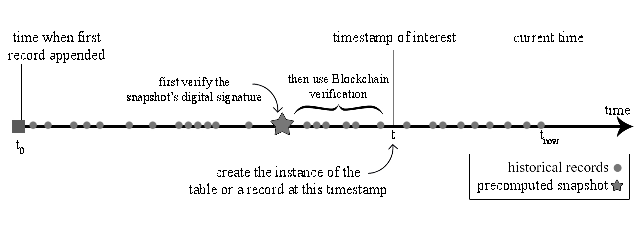
\includegraphics[width=\textwidth]{figs/trusted_snapshot_materialization.pdf}
				\caption{verify trustworthiness of the records in snapshot materialization}
				\label{fig:blockchain_snapshot_materialization}
			\end{figure}

			The remaining issue is that, to digitally sign the records in $s$, we need to make sure about the trustworthiness of the records in the snapshot beforehand. Therefore we propose the following rules for that purpose:

			\begin{itemize}
				\item The first snapshot's records trustworthiness is checked using blockchain verification.
				\item The subsequent snapshots materialize their previous snapshot, hence we take the same steps that was proposed in Definition \ref{defn:trusted_snapshot}.
			\end{itemize}

			Figure \ref{fig:signing_snapshots} depicts the rules that needs to be followed when signing a precomputed snapshot.

			\begin{figure}
				\centering
				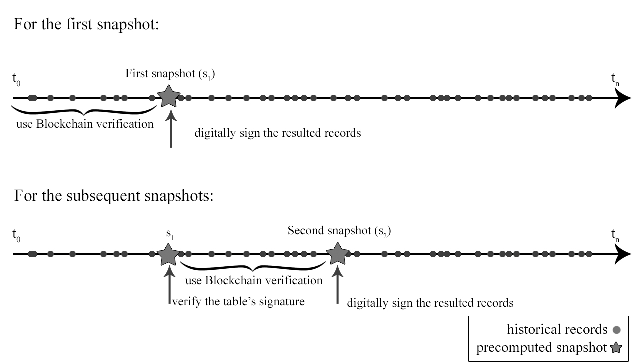
\includegraphics[width=\textwidth]{figs/signing_snapshots.pdf}
				\caption{rules that needs to be followed when signing precomputed snapshots}
				\label{fig:signing_snapshots}
			\end{figure}



	\section{Discussion} \label{sec:algorithm_discussion}

		Utilizing Blockchain technology to provide verifiablilty and immutability for the records that are stored in a temporal relation  discussed in this chapter. We presented a way to store security information of the transactions also known as proof of work to the temporal relations. this is basically achieved by adding the information of the transaction submitter along with the digital signature of the transaction using submitter's cryptogrphic keys. Digital signature of the transactions enables all the users who have access to the public key of the submitters to verify whether or not the submitted records are authenticate or not.

		Although digital signatures grant verifiability of the records but the tables with the security information are still vulnerable to malicious attacks. For example, a super user of the database who can bypass all the security requirements can still perform unverifiable malicious attacks. Therefore, it is naive to assume that using merely the digital signatures can guarantee the trustworthiness of the records. 
		
		To solve the issue, we proposed chaining the submitted records together using their digital signature. This could be done by using the Blockchain technology in which the data are represented in the form of blocks and each block contains the digital signature of their previously submitted block. Any changes on the blocks result in a completely different signature that brings inconsistancy in the chain of digital signatures. To implement this idea, we proposed to add the $previousSignature$ attribute to the records in the temporal table that contains the digital signature of their previous record.

		In order to verify the chain of digital signatures, each record in the temporal relation need to be visited and the correctness of their digital signature as well as the correctness of their previous record's digital signature needs to be investigated. We call this the manual blockchain verification method which is a linear pocess. 

		Also, given a temporal relation which contains historical data of the database, for the sake of decision making and data analytics, it is common to query for the version of the relation in an specific timestamp. These queries could be answered by creating the snapshot of the relation until that timestamp. The process of snapshot creation is also linear as all the records that fall before the query timestamp needs to visited once and the updates on them needs to be applied.

		In this chapter, We reasoned that answering to snapshot creation queries and manual blockchain verification is expensive and inefficient, therefore we proposed to place $m$ number of snapshots for materialization. These snapshots indicate the latest version of a database until that specific timestamp. Note that $m$ which is the number of snapshots to be generated and placed for materialization is determined by checking the available resources of the host system.

		To find optimal locations for placing snapshots, we proposed to store the timestamp of the previous queries on the database to have the patterns of the queries on the timeline. Pattern of the queries gives us the ability to identify the hotspots on the timeline. We argued that it is highly likeley that the the subsequent queries to be performed in these hotspots. in order to solve the problem of finding optimal locations for the snapshots, we proposed to create optimal segmentations of the previously performed queries and allocate an exclusive snapshot for each segmentation for materialization. In this case, when a query falls in the boundaries of a segmentation, it materializes the snapshot of that segmentation.

		In order to find $m$ number of optimal segmentation, we first solved the problem of finding an optimal position to place a single snapshot. We mathematically proved that the optimal place for a single snapshot is the median of the queries, hence if $m$ number of segmentations were created, the optimal position to place snapshot within each segmentation is the median of that segmentation queries. In the next step, we utilized three different methods to find multiple optimal segmentation of queries: recursive algorithm, dynamic programming and heuristic method. In theory, the recursive algorithm consumes the highest computational time among the other two methods. Also, computationally, heuristic method has the lowest computational time complexity over recursive algorithm and dynamic programming, but the optimal solution to the problem is not always guaranteed. In the next chapter we design multiple experiments to evaluate the performance of each method in different scenarios.

		With the intention of providing trusted query results, we proposed to create the digital signatures of the snapshots and append it to the end of the snapshot table. Digitally signing the precomputed snapshots requires to investigate the authenticity of their records before signing them. This process requires manual blockchain verification which is costly, especially for the snapshots that fall at the end of the timeline. In order to save the computational time, we proposed that only the first snapshot use the manual Blockchain verification and the subsequent snapshots use the materialized Blockchain verification using their previous precomputed snapshot. 

